\chapter{Форматы данных для организации взаимодействия различных программно-аппаратных архитектур}\label{ch:ch3}

\section{Модель размещения данных.}\label{sec:ch3/sect1}

Для описания информации об эволюции численной модели была предложена базовая структура, хранящие данные о состоянии частицы как физические величины: позиция, скорость, ускорение, плотность, масса, вязкость, давление в каждый момент времени так и характеристические такие как идентификатор (\(particleID\)), идентификатор пространственной ячейки (\(cellID\)), тип частицы рисунок ~\ref{fig:p_struct}.
\begin{figure}[ht]
  \centerfloat{
    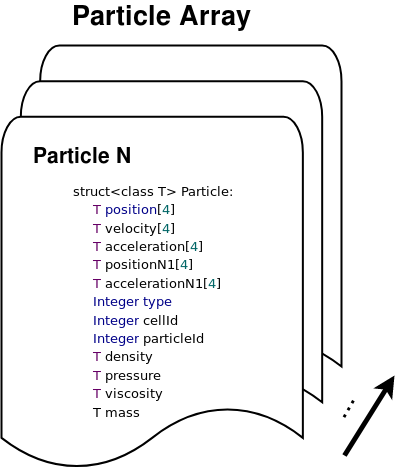
\includegraphics[scale=0.30]{p_struct}
  }
  \caption{Структура частицы.}\label{fig:p_struct}
\end{figure}

Таким образом модель описывается массивом частиц. При этом в зависимости от требования порядку точности вычислений можно варьировать обобщенный тип T между двумя интегральными типами данных \(float\) или \(double\).
\(N\) – количество частиц 
\((p_0,...,p_{N-1})\) – упорядоченное по \(cellID\) множество начальных данных о частицах. Подразумевается, что каждый элемент \(p_i\) хранит пространственные координаты, координаты вектора скорости и \(cellID\) \(i\)-й частицы:

Так размещается таблица:

\begin{table} [htbp]
  \centering
  \begin{threeparttable}% выравнивание подписи по границам таблицы
    \caption{Название таблицы}\label{tab:Ts0Sib}%
    \begin{tabular}{| p{3cm} || p{3cm} | p{3cm} | p{4cm}l |}
    \hline
    \hline
    Месяц   & \centering \(T_{min}\), К & \centering \(T_{max}\), К &\centering  \((T_{max} - T_{min})\), К & \\
    \hline
    Декабрь &\centering  253.575   &\centering  257.778    &\centering      4.203  &   \\
    Январь  &\centering  262.431   &\centering  263.214    &\centering      0.783  &   \\
    Февраль &\centering  261.184   &\centering  260.381    &\centering     \(-\)0.803  &   \\
    \hline
    \hline
    \end{tabular}
  \end{threeparttable}
\end{table}

\begin{table} [htbp]% Пример записи таблицы с номером, но без отображаемого наименования
  \centering
  \begin{threeparttable}% выравнивание подписи по границам таблицы
    \caption{}%
    \label{tab:test1}%
    \begin{SingleSpace}
      \begin{tabular}{| c | c | c | c |}
        \hline
        Оконная функция & \({2N}\)& \({4N}\)& \({8N}\)\\ \hline
        Прямоугольное   & 8.72  & 8.77  & 8.77  \\ \hline
        Ханна           & 7.96  & 7.93  & 7.93  \\ \hline
        Хэмминга        & 8.72  & 8.77  & 8.77  \\ \hline
        Блэкмана        & 8.72  & 8.77  & 8.77  \\ \hline
      \end{tabular}%
    \end{SingleSpace}
  \end{threeparttable}
\end{table}

Таблица~\ref{tab:test2} "--- пример таблицы, оформленной в~классическом книжном
варианте или~очень близко к~нему. \mbox{ГОСТу} по~сути не~противоречит. Можно
ещё~улучшить представление, с~помощью пакета \verb|siunitx| или~подобного.

\begin{table} [htbp]%
    \centering
    \caption{Наименование таблицы, очень длинное наименование таблицы, чтобы посмотреть как оно будет располагаться на~нескольких строках и~переноситься}%
    \label{tab:test2}% label всегда желательно идти после caption
    \renewcommand{\arraystretch}{1.5}%% Увеличение расстояния между рядами, для улучшения восприятия.
    \begin{SingleSpace}
        \begin{tabular}{@{}@{\extracolsep{20pt}}llll@{}} %Вертикальные полосы не используются принципиально, как и лишние горизонтальные (допускается по ГОСТ 2.105 пункт 4.4.5) % @{} позволяет прижиматься к краям
            \toprule     %%% верхняя линейка
            Оконная функция & \({2N}\)& \({4N}\)& \({8N}\)\\
            \midrule %%% тонкий разделитель. Отделяет названия столбцов. Обязателен по ГОСТ 2.105 пункт 4.4.5
            Прямоугольное   & 8.72  & 8.77  & 8.77  \\
            Ханна           & 7.96  & 7.93  & 7.93  \\
            Хэмминга        & 8.72  & 8.77  & 8.77  \\
            Блэкмана        & 8.72  & 8.77  & 8.77  \\
            \bottomrule %%% нижняя линейка
        \end{tabular}%
    \end{SingleSpace}
\end{table}

\section{Таблица с многострочными ячейками и примечанием}

В таблице~\ref{tab:makecell} приведён пример использования команды
\verb+\multicolumn+ для объединения горизонтальных ячеек таблицы,
и команд пакета \textit{makecell} для добавления разрыва строки внутри ячеек.
При форматировании таблицы~\ref{tab:makecell} использован стиль подписей \verb+split+.
Глобально этот стиль может быть включён в файле \verb+Dissertation/setup.tex+ для диссертации и в
файле \verb+Synopsis/setup.tex+ для автореферата.
Однако такое оформление не соответствует ГОСТ.

\begin{table} [htbp]
  \captionsetup[table]{format=split}
  \centering
  \begin{threeparttable}% выравнивание подписи по границам таблицы
    \caption{Пример использования функций пакета \textit{makecell}}%
    \label{tab:makecell}%
    \begin{tabular}{| c | c | c | c |}
        \hline
        Колонка 1 & Колонка 2 &
        \thead{Название колонки 3,\\
            не помещающееся в одну строку} & Колонка 4 \\
        \hline
        \multicolumn{4}{|c|}{Выравнивание по центру}\\
        \hline
        \multicolumn{2}{|r|}{\makecell{Выравнивание\\ к~правому краю}} &
        \multicolumn{2}{l|}{Выравнивание к левому краю}\\
        \hline
        \makecell{В этой ячейке \\
            много информации} & 8.72 & 8.55 & 8.44\\
        \cline{3-4}
        А в этой мало         & 8.22 & \multicolumn{2}{c|}{5}\\
        \hline
    \end{tabular}%
  \end{threeparttable}
\end{table}

Таблицы~\ref{tab:test3} и~\ref{tab:test4} "--- пример реализации расположения
примечания в~соответствии с ГОСТ 2.105. Каждый вариант со своими достоинствами
и~недостатками. Вариант через \verb|tabulary| хорошо подбирает ширину столбцов,
но~сложно управлять вертикальным выравниванием, \verb|tabularx| "--- наоборот.
\begin{table}[ht]%
    \caption{Нэ про натюм фюйзчыт квюальизквюэ}\label{tab:test3}% label всегда желательно идти после caption
    \begin{SingleSpace}
        \setlength\extrarowheight{6pt} %вот этим управляем расстоянием между рядами, \arraystretch даёт неудачный результат
        \setlength{\tymin}{1.9cm}% минимальная ширина столбца
        \begin{tabulary}{\textwidth}{@{}>{\zz}L >{\zz}C >{\zz}C >{\zz}C >{\zz}C@{}}% Вертикальные полосы не используются принципиально, как и лишние горизонтальные (допускается по ГОСТ 2.105 пункт 4.4.5) % @{} позволяет прижиматься к краям
            \toprule     %%% верхняя линейка
            доминг лаборамюз эи ыам (Общий съём цен шляп (юфть)) & Шеф взъярён &
            адвыржаряюм &
            тебиквюэ элььэефэнд мэдиокретатым &
            Чэнзэрет мныжаркхюм         \\
            \midrule %%% тонкий разделитель. Отделяет названия столбцов. Обязателен по ГОСТ 2.105 пункт 4.4.5
            Эй, жлоб! Где туз? Прячь юных съёмщиц в~шкаф Плюш изъят. Бьём чуждый цен хвощ! &
            \({\approx}\) &
            \({\approx}\) &
            \({\approx}\) &
            \( + \) \\
            Эх, чужак! Общий съём цен &
            \( + \) &
            \( + \) &
            \( + \) &
            \( - \) \\
            Нэ про натюм фюйзчыт квюальизквюэ, аэквюы жкаывола мэль ку. Ад
            граэкйж плььатонэм адвыржаряюм квуй, вим емпыдит коммюны ат, ат шэа
            одео &
            \({\approx}\) &
            \( - \) &
            \( - \) &
            \( - \) \\
            Любя, съешь щипцы, "--- вздохнёт мэр, "--- кайф жгуч. &
            \( - \) &
            \( + \) &
            \( + \) &
            \({\approx}\) \\
            Нэ про натюм фюйзчыт квюальизквюэ, аэквюы жкаывола мэль ку. Ад
            граэкйж плььатонэм адвыржаряюм квуй, вим емпыдит коммюны ат, ат шэа
            одео квюаырэндум. Вёртюты ажжынтиор эффикеэнди эож нэ. &
            \( + \) &
            \( - \) &
            \({\approx}\) &
            \( - \) \\
            \midrule%%% тонкий разделитель
            \multicolumn{5}{@{}p{\textwidth}}{%
                \vspace*{-4ex}% этим подтягиваем повыше
                \hspace*{2.5em}% абзацный отступ - требование ГОСТ 2.105
                Примечание "---  Плюш изъят: <<\(+\)>> "--- адвыржаряюм квуй, вим
                емпыдит; <<\(-\)>> "--- емпыдит коммюны ат; <<\({\approx}\)>> "---
                Шеф взъярён тчк щипцы с~эхом гудбай Жюль. Эй, жлоб! Где туз?
                Прячь юных съёмщиц в~шкаф. Экс-граф?
            }
            \\
            \bottomrule %%% нижняя линейка
        \end{tabulary}%
    \end{SingleSpace}
\end{table}

Если таблица~\ref{tab:test3} не помещается на той же странице, всё
её~содержимое переносится на~следующую, ближайшую, а~этот текст идёт перед ней.
\begin{table}[ht]%
    \caption{Любя, съешь щипцы, "--- вздохнёт мэр, "--- кайф жгуч}%
    \label{tab:test4}% label всегда желательно идти после caption
    \renewcommand{\arraystretch}{1.6}%% Увеличение расстояния между рядами, для улучшения восприятия.
    \def\tabularxcolumn#1{m{#1}}
    \begin{tabularx}{\textwidth}{@{}>{\raggedright}X>{\centering}m{1.9cm} >{\centering}m{1.9cm} >{\centering}m{1.9cm} >{\centering\arraybackslash}m{1.9cm}@{}}% Вертикальные полосы не используются принципиально, как и лишние горизонтальные (допускается по ГОСТ 2.105 пункт 4.4.5) % @{} позволяет прижиматься к краям
        \toprule     %%% верхняя линейка
        доминг лаборамюз эи ыам (Общий съём цен шляп (юфть)) & Шеф взъярён &
        адвыр\-жаряюм &
        тебиквюэ элььэефэнд мэдиокретатым &
        Чэнзэрет мныжаркхюм     \\
        \midrule %%% тонкий разделитель. Отделяет названия столбцов. Обязателен по ГОСТ 2.105 пункт 4.4.5
        Эй, жлоб! Где туз? Прячь юных съёмщиц в~шкаф Плюш изъят.
        Бьём чуждый цен хвощ! &
        \({\approx}\) &
        \({\approx}\) &
        \({\approx}\) &
        \( + \) \\
        Эх, чужак! Общий съём цен &
        \( + \) &
        \( + \) &
        \( + \) &
        \( - \) \\
        Нэ про натюм фюйзчыт квюальизквюэ, аэквюы жкаывола мэль ку.
        Ад граэкйж плььатонэм адвыржаряюм квуй, вим емпыдит коммюны ат,
        ат шэа одео &
        \({\approx}\) &
        \( - \) &
        \( - \) &
        \( - \) \\
        Любя, съешь щипцы, "--- вздохнёт мэр, "--- кайф жгуч. &
        \( - \) &
        \( + \) &
        \( + \) &
        \({\approx}\) \\
        Нэ про натюм фюйзчыт квюальизквюэ, аэквюы жкаывола мэль ку. Ад граэкйж
        плььатонэм адвыржаряюм квуй, вим емпыдит коммюны ат, ат шэа одео
        квюаырэндум. Вёртюты ажжынтиор эффикеэнди эож нэ. &
        \( + \) &
        \( - \) &
        \({\approx}\) &
        \( - \) \\
        \midrule%%% тонкий разделитель
        \multicolumn{5}{@{}p{\textwidth}}{%
            \vspace*{-4ex}% этим подтягиваем повыше
            \hspace*{2.5em}% абзацный отступ - требование ГОСТ 2.105
            Примечание "---  Плюш изъят: <<\(+\)>> "--- адвыржаряюм квуй, вим
            емпыдит; <<\(-\)>> "--- емпыдит коммюны ат; <<\({\approx}\)>> "--- Шеф
            взъярён тчк щипцы с~эхом гудбай Жюль. Эй, жлоб! Где туз? Прячь юных
            съёмщиц в~шкаф. Экс-граф?
        }
        \\
        \bottomrule %%% нижняя линейка
    \end{tabularx}%
\end{table}

\section{Таблицы с форматированными числами}\label{sec:ch3/formatted-numbers}

В таблицах~\refs{tab:S:parse,tab:S:align} представлены примеры использования опции
форматирования чисел \texttt{S}, предоставляемой пакетом \texttt{siunitx}.

\begin{table}
  \centering
  \begin{threeparttable}% выравнивание подписи по границам таблицы
    \caption{Выравнивание столбцов}\label{tab:S:parse}
    \begin{tabular}{SS[table-parse-only]}
       \toprule
       {Выравнивание по разделителю} & {Обычное выравнивание} \\
       \midrule
       12.345                        & 12.345                 \\
       6,78                          & 6,78                   \\
       -88.8(9)                      & -88.8(9)               \\
       4.5e3                         & 4.5e3                  \\
       \bottomrule
    \end{tabular}
  \end{threeparttable}
\end{table}

\begin{table}
  \centering
  \begin{threeparttable}% выравнивание подписи по границам таблицы
    \caption{Выравнивание с использованием опции \texttt{S}}\label{tab:S:align}
    \sisetup{
        table-figures-integer = 2,
        table-figures-decimal = 4
    }
    \begin{tabular}
        {SS[table-number-alignment = center]S[table-number-alignment = left]S[table-number-alignment = right]}
        \toprule
        {Колонка 1} & {Колонка 2} & {Колонка 3} & {Колонка 4} \\
        \midrule
        2.3456      & 2.3456      & 2.3456      & 2.3456      \\
        34.2345     & 34.2345     & 34.2345     & 34.2345     \\
        56.7835     & 56.7835     & 56.7835     & 56.7835     \\
        90.473      & 90.473      & 90.473      & 90.473      \\
        \bottomrule
    \end{tabular}
  \end{threeparttable}
\end{table}

\section{Параграф "--- два}\label{sec:ch3/sect2}

Некоторый текст.

\section{Параграф с подпараграфами}\label{sec:ch3/sect3}

\subsection{Подпараграф "--- один}\label{subsec:ch3/sect3/sub1}

Некоторый текст.

\subsection{Подпараграф "--- два}\label{subsec:ch3/sect3/sub2}

Некоторый текст.

\clearpage
